\documentclass{article}

\usepackage{graphicx}
\usepackage{listings}

\graphicspath{./}

\begin{document}
    \title  { \textbf{SYSC 4602 Assignment 4} }
    \author {
        David Song (101071234)\\
        Ghassan Arnouk (101078550)\\
        Zachary Porter (101069001)
    }

    \maketitle

    \clearpage
    \section*{Part 3: IP Packet Structure}
    \subsection*{1}
    IP address of our computer: 172.17.59.194\\
    IP address of remote server: 5.9.243.187\\
    \subsection*{2}
    Yes the total length field includes the header size.\\
    The header size is 20 bytes, the pyload size is 40 bytes and the total length is 60 bytes.\\
    \subsection*{3}
    The identification field changes for each packet. The identification field in packets being sent start from 0x5442, and increase in value by 1 for each subsiquent packet. This allows the packets to be reordered if they arrive out of order. With packets being received the identification field starts at 0x4403 and increases for each subsiquent packet.
    \subsection*{4}
    The TTL field on packets sent from our computer is not its maximum value of 256 (0xFF). It is a lower value of 64 (0x40)
    \subsection*{5}
    The flags indicate if the packet has been fragmented, and the fragment offset will indicate fragmentation aswell.\\
    In our trace the flags indicate not to fragment and the fragmentation offset is 0.
    \subsection*{6}
    The header length is 20 bytes.
    \begin{figure}[htbp]
        \centering
        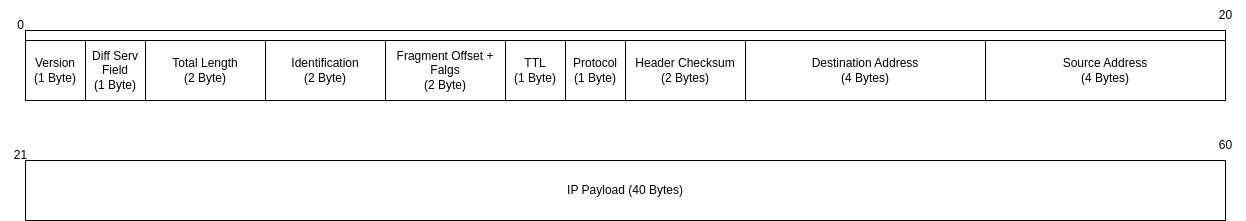
\includegraphics[width=\textwidth]{images/part3.drawio.png}
        \caption{IP Packet Structure}
    \end{figure}
    \section*{Part 4: Internet Paths}
    \lstinputlisting[caption=Traceroute output]{traces/traceroute.log}
    \clearpage
    \begin{figure}[htbp]
        \centering
        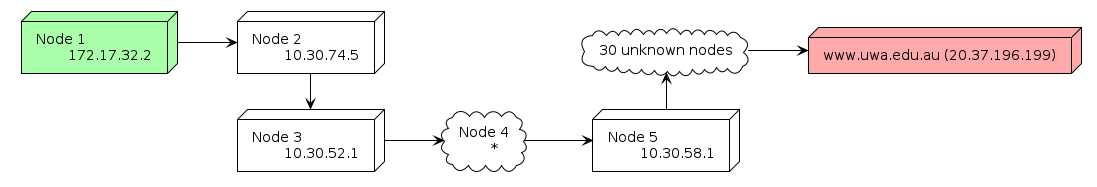
\includegraphics[width=\textwidth]{images/part4.plantuml.png}
        \caption{Network map diagram based on traceroute}
    \end{figure}
    \section*{Part 5: IP Header Checksum}
    \subsection*{1}
    4500 058c 4407 4000 2b06 25cd 0509 f3bb ac11 3bc2
    \subsection*{2}
    Result of addition is 2FFFD
    \subsection*{3}
    1's Complement is FFFF
    \subsection*{4}
    The result is as expected, 0 in 1's Complement form.
\end{document}
